\section{Case Study}
\label{sec:casestudy}
A design and fabrication workshop was organized to examine the feasibility of our system with a specific design target and a location.
We selected a public community house where people in the community share the space and regularly use the facility.
Participants of the workshop were selected among them, who were four children aged 10 and under (4, 7, 9 , and 10 years old) and two parents (Figure~\ref{fig:workshop}).
We specifically selected children with this range of age as non-experts without experiences in computational design or digital fabrication, also for observing the clarity and attractiveness of the game.
The entire workshop was filmed and documented in a short clip.
Please refer the supplementary video material for the documentation.

The goal for the participants was to contribute to an ongoing design and fabrication process of screen wall (2m by 0.9m) consisting of 8 rectangles.
Six frames were already designed and built, thus the rest two frames were prioritized for them to design and fabricate in this workshop.

Participants were informed about the goal of the workshop, and each process was introduced by experienced tutors.
The processes were from collecting and fixing the branches on a plate, scanning the plate, complete designs by playing the game, and assembly after CNC milling.

\begin{figure}[ht]
  \begin{center}
    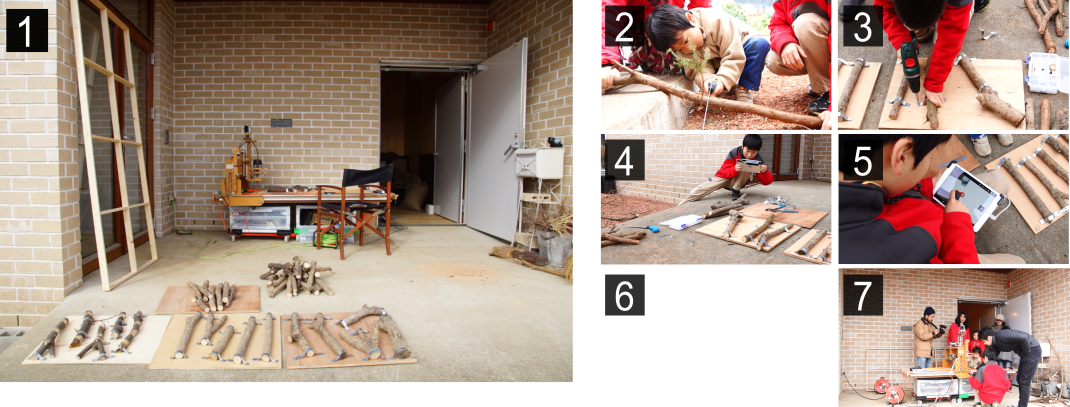
\includegraphics[width = 0.4\paperwidth]{images/fabrication/workshop_setup.png}
    \caption{An overview of the workshop. 1.the overview of the space. 2.collect branches. 3.cut in certain lengths 4.attach on a plate 5.scan the plate 6.play the game 7.CNC milling.}
    \label{fig:workshop}
  \end{center}
\end{figure}

\subsection{Setup}
\subsubsection*{System and Hardware Setup}
We used two iPad-minis with iSense depth cameras attached for scanning branches, and a 3 axis CNC milling router with a 6 mm diameter milling bit.
We used a laptop PC (Lenovo w240 with intel core i7) for running \textit{Branch Importer} and \textit{G-Code generator}, as well as operating the milling machine.
The scan area of iSense camera is 500mm x 500mm, and the milling machine's stroke length along z-axis is 70mm, which provide geometric constraints for available branch sizes.
\textit{BranchConnect} was hosted at \textit{Heroku} cloud server \footnote{ Heroku is a platform as a service (PaaS) that enables developers to build, run, and operate applications entirely in the cloud. \url{https://www.heroku.com/}},
and we used \textit{MongoDB} \footnote{ MongoDB is a free and open-source cross-platform document-oriented database program. \url{https://www.mongodb.com/}} as a cloud database.

\subsubsection*{Preparation of Branches}
The participants were asked to collect branches with 2 - 10 cm in diameter.
The lower bound of the diameter was set due to the milling bit size, and the upper bound was set for the limited length of z-stroke of the CNC router.
The collected branches were cut in arbitrary lengths, not longer than 500 mm due to the limit of scanning area. \\

As our game system and fabrication process take 3D branch shapes as 2D contours (with limited use of point cloud), these constraints work positive for the system which automatically filter out branches with large 3D twists.
We asked participants to scan with iPad + iSense and prepare feasible mesh model by themselves.
After obtaining mesh models, tutors imported models from iPads to a laptop and upload them to database by \textit{Branch Importer}.


\subsubsection*{User Experiences with the System}
After models are uploaded to the server, users can see that their plates are added in the selectable branch plates with their names and locations.
Users can access to the start page by PC and mobile devices.
We prepare both options and let participants choose a device.

A user is firstly directed to a start page and asked to submit a user name.
Secondly, the user is navigated to target frame selection page, and asked to pick one out of eight frames.
Each frame has different target points.
The interface also shows the completed branch organizations within each target frame.
If there are multiple designs, three designs with highest scores are displayed.
The user can change the currently displayed design by clicking within each frame and choose either starting their design from scratch, or select the design and improve it.

After selecting a target frame, the user goes to branch selection page, displaying 15 plates when the workshop was held.
In this page, they see the plates made by themselves on the page, as well as their names on the plate.
The user can select the same plate for designing other target frames.
By clicking a displayed branch plate, the user is navigated to the game interface.
After completing to bridge all the target points, the design is automatically uploaded to the database, but the use can continue to design.
Tutors and participants select layout design for the assigned two target frames, and an experienced tutor operates \textit{G-Code Generator} as well as the CNC router.
Participants were asked to assembly branches after joineries were milled.

\subsection{Results}
The entire workshop took 4.6 hours to complete the whole process, including introduction, moving, and pauses.
Table \ref{tab:timing} shows durations of each task.

\begin{center}
  \begin{tabulary}{\columnwidth}{ |l||C|C| }
    \hline
    Task & Duration (hour) & Fraction ($\%$) \\
    \hline
    Introduction                  & 0.3 & 6.5  \\
    Collecting branches           & 0.6 & 13.0  \\
    Preparing plates              & 0.8 & 17.4  \\
    Preparing models              & 0.3 & 6.5  \\
    Uploading models              & 0.2 & 4.3 \\
    Designing by the game         & 0.5 & 10.8 \\
    Inspecting models             & 0.2 & 4.3 \\
    CNC milling                   & 0.5 & 10.8\\
    Assembling                    & 0.2 & 4.3 \\
    Moving, pauses               & 1.0 & 21.7 \\
    \hline
    In total                      & 4.6   & 100 \\
    \hline
  \end{tabulary}
  \label{tab:timing}
\end{center}

\subsubsection*{Collecting Branches}
The diameter and length constraints for available branches worked as guidelines for participants rather than restricting finding and cutting arbitrary branches.
After cutting branches in certain lengths, participants fixed branches on plates by thin metal plates with screw holes.
It was straightforward for them to firmly fix branches so that they are not moved during milling process.
These fixture points are counted as invalid points in the game where joinery points can not be generated.
The participants built two plates with three and five branches fixed on each plate.

\subsubsection*{Model Acquisition}
iSense camera comes with an intuitive software for scanning and modifying models.
After we gave an instruction, most of participants practiced several scans and successfully scanned models without any problem.

Each scanning and re-touching took 2-3 minutes, and 30 seconds for generating data by \textit{Branch Importer}.
Including the prepared panels previously, we scanned 15 plates in total, 75 branches, and 35.3m of total length including sub-branches.
We got 59 branches with a single skeleton, 16 branches with multiple skeletons for grafting.
The result is shown in Figure \ref{fig:scannedplates}.

\begin{figure}[ht]
  \begin{center}
    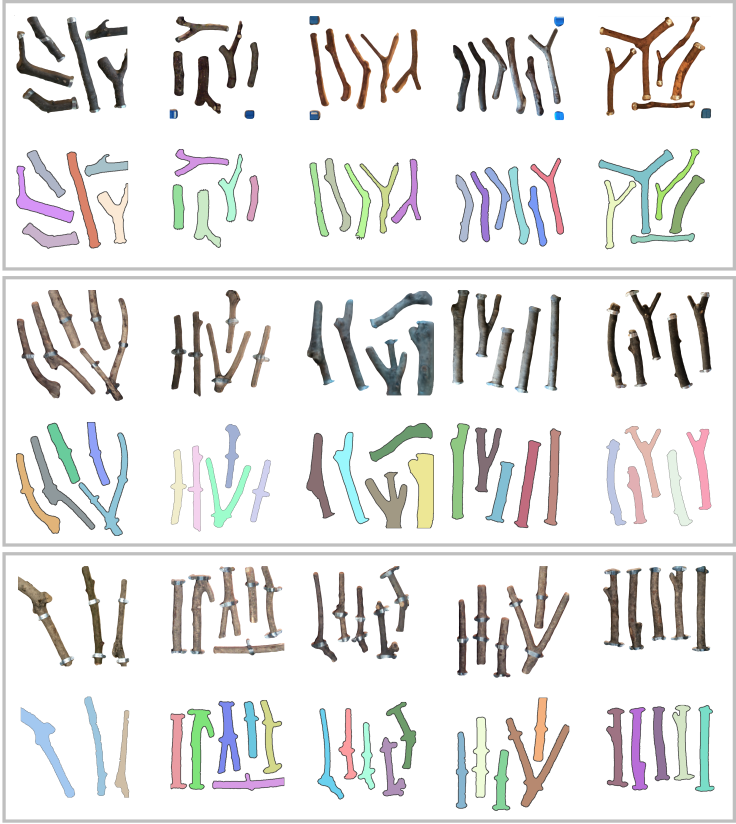
\includegraphics[width = 0.4\paperwidth]{images/fabrication/all_plates.png}
    \caption{An overview of all the 15 scanned plates for the construction of the fence. Top raw of each set shows ortho-top views of scanned mesh models, and the bottom raw is the recognized branches with randomly assigned colors. The red-lined rectangles indicate the plates built by participants in the workshop.}
    \label{fig:scannedplates}
  \end{center}
\end{figure}


\subsubsection*{Design with the Game}
Most participants used iPads for navigating pages and playing the game.
All the participants understood the goal immediately, however, they had difficulties with mobile touch interface, such as rotation and flipping operation by gestures.

One participant switched to play by a PC for more precise control due to the problem.
All the participants chose to develop their own designs from the scratch, although they had instruction about the "continue existing designs".

Although there is no time limit in the game system, we set 30 minutes for playing the game, and 8 layout designs were given by participants.
2 frames were completed per participants and 2 participants completed the whole eight target frames.
The average score was xxx, and average playing duration was xxx to complete each target frame.

\subsubsection*{Global Design Consensus}
As the target frame selection page can display designs not only from one user but also from all the others at once, we could get an overview of design options.
The layout designs were displayed as score descending order with limited numbers (3 highest scores), we could find feasible layout designs easily with mostly all the target points were bridged.
As participants were excited by seeing their branches and designs, we took two invalid layout designs and one plate which did not have enough branches for the global design.

\subsubsection*{Fabrication}
We did not have major problems for converting designs to G-Code milling paths as we encountered major issues regarding the fabrication before the workshop, which are reported in this section.

The main problem was the accuracy of acquired contours.
We observed most of scanned models had occluded regions between plates and branches, which create interpolated faces during solidifying process, resulting in outwardly offsetted contours. \todo{check offsetted correct english} After milling was finished and when branches were assembled, six pairs of branches were loosely connected because the calculated contours were 2-3mm eroded than the actual sizes.
We avoided this problem by trimming branches from 2-5 mm higher than the plate surface.
After this operation, the rest of connections were tightly connected. \\

We also observed that many milling paths were 5-10 mm off from the center of planned joints.
Multiple reasons could be considered as reasons such as,

\begin{itemize}
  \item{deformation of mechanical parts of the CNC router}
  \item{not dense resolution of acquired contours of branches}
  \item{misaligned orientation of the plate compared to the scanned model}
\end{itemize}

To avoid the misalignments, we modified the \textit{G-Code Generator} so that an operator can freely adjust the absolute origin of the generated milling paths.
The origin was usually set with around the center of the plate.
After this modification, the misalignment from joint center was reduced with 5 mm off at the maximum misalignment.
Branches could absorb 3-5 mm misaligned joint positions due to the elasticity of branches, and solidifying the structure with residual stresses from misalignments.
% The misaligned joint positions worked as post-tensions, solidifying the structure.
% We assume that this is only applicable when an applied bending moment and cut surface at a joint is orthogonal or not too much off from orthogonal. \todo{this sentence}



\subsection{Summary of the Case Study}
% \subsubsection*{Organization of the Workshop}
The objective of the workshop was to observe the validity of our system for non-expert users.
We could see that participants aged 10 and under were capable of following the workflow.
Participants were encouraged to contribute to the ongoing design with the online platform, and successfully provided designs from available branch plates.

We had several requests from participants regarding the game interface but also related to the workshop organization. Several participants requested to allow multiple branch plates for designing a frame, or even remove the target frame and let them freely design with branches.
Also a participant who gave up with iPad operations requested additional buttons for mobile touch interface to keep an active branch selected.

The participant with four years old failed to complete the game, however, insisted on accepting his design to be fabricated.
Similarly a branch plate made by another participant had only three branches, which is not enough to fulfill bridging target points.
We took them as positive inputs to validate our participatory (architectural) design approach.
